% CRSP: Cognition via Rewarded Self-Play

\documentclass[10pt,a4paper]{article}
\usepackage[margin=1in]{geometry}
\usepackage{amsmath}
\usepackage{amssymb}
\usepackage{amsfonts}
\usepackage{graphicx}
\usepackage{algorithm}
\usepackage{algorithmic}
\usepackage{hyperref}
\usepackage{verbatim}
\usepackage{fancyhdr}
\usepackage{setspace}
\setlength{\headheight}{14pt}
\usepackage[T1]{fontenc}
\usepackage[default]{sourcesanspro}  % Modern sans-serif font for main text
\usepackage[mono]{roboto-mono}  % Modern monospace font
\usepackage{sourcecodepro}  % Modern monospace font for titles
\usepackage{tikz}      % For creating diagrams
\usetikzlibrary{shapes.geometric, arrows, positioning, calc}
\usetikzlibrary{arrows.meta}  % For better arrow styles

% Fine-tune the font settings
\renewcommand{\familydefault}{\sfdefault}
\linespread{1.05}  % Slightly increase line spacing for better readability
\usepackage{microtype}  % Better typography
\usepackage{ragged2e}  % Better text alignment
\usepackage{xcolor}    % For colored text

% Set default font to Roboto
\renewcommand{\familydefault}{\sfdefault}
% Set monospace font to Roboto Mono
\renewcommand{\ttdefault}{rtm}

% Make all section titles use Source Code Pro
\makeatletter
\renewcommand\section{\@startsection{section}{1}{\z@}%
  {-3.5ex \@plus -1ex \@minus -.2ex}%
  {2.3ex \@plus.2ex}%
  {\fontfamily{sourcecodepro}\selectfont\Large\bfseries}}
\renewcommand\subsection{\@startsection{subsection}{2}{\z@}%
  {-3.25ex\@plus -1ex \@minus -.2ex}%
  {1.5ex \@plus .2ex}%
  {\fontfamily{sourcecodepro}\selectfont\large\bfseries}}
\renewcommand\subsubsection{\@startsection{subsubsection}{3}{\z@}%
  {-3.25ex\@plus -1ex \@minus -.2ex}%
  {1.5ex \@plus .2ex}%
  {\fontfamily{sourcecodepro}\selectfont\normalsize\bfseries}}
\makeatother

% Ensure text is left-aligned by default
\raggedright

% Custom formatting for a professional look
\pagestyle{fancy}
\fancyhf{}
\fancyhead[L]{CRSP: Cognition via Rewarded Self-Play}
\fancyhead[R]{\thepage}
\renewcommand{\headrulewidth}{0.4pt}

% Adjust spacing
\setstretch{1.1}

% Custom environment for prompt boxes
\usepackage{tcolorbox}
\newtcolorbox{promptbox}[1]{
    colback=white,
    colframe=black,
    boxrule=1pt,
    arc=2pt,
    left=5pt,
    right=5pt,
    top=5pt,
    bottom=5pt,
    title=#1,
    fonttitle=\bfseries,
    coltitle=black,
    colbacktitle=gray!20
}

% Custom title page without centering
\makeatletter
\def\@maketitle{%
  \newpage
  \null
  \vspace{2em}%
  {\raggedright\huge\fontfamily{sourcecodepro}\selectfont\bfseries\@title\par}%
  \vspace{1.5em}%
  {\raggedright\normalsize\bfseries\@author\par}%
  \vspace{1em}%
  \vspace{2em}%
}
\makeatother

\title{Cognition via Rewarded Self-Play: Open-Ended Emergent Reasoning Through Guided Self-Search}
\author{
    {\small\textbf{Netanel Benisti}}\\[0.1em]
    {\small\textmd{Recursive Intelligence}}\\[0.1em]
    {\small\color{gray}\textmd{recursive-intelligence@proton.me}}
}
\date{\today}

\begin{document}

% Define custom header style for first page
\fancypagestyle{firstpage}{%
    \fancyhf{}% Clear all header and footer fields
    \fancyhead[L]{\includegraphics[height=0.8cm]{logo.png}}%
    \fancyhead[R]{\today}%
    \renewcommand{\headrulewidth}{0.4pt}%
}

\maketitle
\thispagestyle{firstpage}

\vspace{1cm}

% Redefine abstract environment to be left-aligned
\renewenvironment{abstract}
 {\par\noindent{\fontfamily{sourcecodepro}\selectfont\Large\mdseries\textbf{Abstract}}\par\vspace{1em}\noindent}
 {\par\vspace{1em}}

\begin{abstract}
We introduce \textbf{Cognition via Rewarded Self-Play (CRSP)}, a framework for recursive self-improvement that enables open-ended reasoning through guided self-search at the edge of chaos. CRSP follows a two-phase architecture: an initial \textit{Trajectory Seeding} stage grounds cognition using high-fidelity LIMO traces, followed by autonomous development through strategic task synthesis. At its core is a three-policy self-play loop that generates tasks of optimal difficulty and rewards the reasoning trajectory itself—captured through chain-of-thought (CoT)—even in the absence of correctness.
This feedback loop drives continual self-improvement: the system proposes increasingly complex challenges, engages in extended deliberation to solve them, and refines its strategies through multi-dimensional critique. In doing so, it conducts a principled, guided search over its own reasoning space. By operating at the edge of chaos, CRSP naturally filters for only the most instructive samples, reducing dependence on large external datasets while achieving superior generalization and reasoning capabilities.
CRSP demonstrates that open-ended cognition emerges when self-search is scaffolded by well-calibrated reward structures—balancing exploration, coherence, and metacognitive reflection. Our approach represents a shift from passive learning on static datasets to an active, self-generating curriculum, where the system iteratively acts as its own teacher, student, and critic in an unbounded loop of cognitive amplification.  
\end{abstract}

\begin{figure}[htbp]
\centering
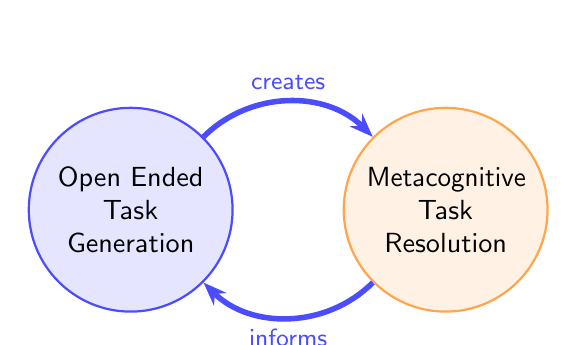
\begin{tikzpicture}[
    node distance=4cm,
    thick,
    every node/.style={align=center},
    task/.style={circle, draw=blue!70, fill=blue!10, minimum size=2.5cm, text width=2cm},
    resolution/.style={circle, draw=orange!70, fill=orange!10, minimum size=2.5cm, text width=2cm},
    arrow/.style={-{Stealth[length=3mm]}, blue!70, line width=2pt}
]

% Nodes
\node[task] (task) {\textmd{Open Ended\\Task\\Generation}};
\node[resolution, right of=task] (resolution) {\textmd{Metacognitive\\Task\\Resolution}};

% Arrows
\draw[arrow, bend left=45] (task) to node[above, blue!70] {\small creates} (resolution);
\draw[arrow, bend left=45] (resolution) to node[below, blue!70] {\small informs} (task);

\end{tikzpicture}
\caption{Core conceptual cycle of CRSP: The system continuously generates open-ended tasks that challenge its reasoning capabilities, then engages in metacognitive task resolution through detailed deliberation and self-critique. The insights gained from this resolution process inform the creation of even more sophisticated tasks, creating a self-reinforcing cycle of cognitive growth and recursive self-improvement.}
\label{fig:crsp_cycle}
\end{figure}

At its heart, CRSP embodies a fundamental cycle of cognitive growth illustrated in Figure~\ref{fig:crsp_cycle}. The system generates open-ended tasks that push the boundaries of its current capabilities, then engages in metacognitive task resolution through extended reasoning and self-critique. This resolution process—involving detailed deliberation, verification, and creative exploration—generates insights that inform the creation of even more sophisticated tasks. This creates a self-reinforcing cycle where each iteration builds upon the lessons learned from previous attempts, enabling continuous cognitive amplification without external supervision.

\begin{figure}[htbp]
\centering
\includegraphics[width=0.8\textwidth]{overall-bot.png}
\caption{CRSP as a self-play metacognitive framework that encourages open-ended reasoning through iterative task generation, solution development, and critical evaluation in a continuous learning loop.}
\label{fig:overall_crsp}
\end{figure}

\textbf{Keywords:} Reinforcement Learning, Self-Play, Reasoning, Language Models, Trajectory Seeding, Reward Modeling

\section{Introduction}

The emergence of sophisticated reasoning capabilities in large language models represents one of the most significant developments in artificial intelligence, yet current approaches face fundamental scalability and generalization challenges. While supervised fine-tuning requires extensive human-annotated reasoning traces, and traditional reinforcement learning from human feedback (RLHF) depends on costly human preference data, recent work has demonstrated that complex reasoning can emerge through self-play mechanisms that eliminate dependence on external supervision~\cite{zhao2025absolute, ye2025emergence}.

This philosophical motivation draws inspiration from biological learning systems, where cognition emerges through iterative hypothesis testing and refinement—a process analogous to guided self-search within the constraints of physical and cognitive limitations. Just as biological systems operate at the "edge of chaos" where optimal learning occurs through balanced exploration and exploitation~\cite{langton1990computation}, artificial reasoning systems require carefully calibrated feedback mechanisms to navigate the vast space of possible reasoning trajectories.

Recent empirical evidence from Zhang et al.~\cite{zhang2024intelligence} demonstrates that optimal machine intelligence emerges precisely at this edge of chaos, where models trained on complex but not chaotic rule systems exhibit superior performance on downstream reasoning tasks. Their findings reveal that models operating at the transition between order and disorder develop sophisticated internal representations that naturally integrate historical information into their reasoning processes, exhibiting extended attention patterns that mirror the lengthy reasoning chains encouraged by CRSP's exploration rewards.

Building on the Absolute Zero Reasoner (AZR) paradigm~\cite{zhao2025absolute}, which demonstrated that reasoning capabilities can emerge through self-play without external data, we propose \textbf{Cognition via Rewarded Self-Play (CRSP)}, a framework that addresses two critical limitations of existing approaches: (1) the lack of high-quality initialization that leverages existing knowledge foundations, and (2) the insufficient reward structure that fails to capture the multi-dimensional nature of reasoning quality.

The theoretical foundation for such self-guided search capabilities is supported by recent work on the Turing completeness of prompting~\cite{qiu2024turing}, which demonstrates that a single finite-size Transformer can compute any computable function given appropriate prompts. This result provides strong theoretical backing for CRSP's approach, suggesting that there is no fundamental computational limitation preventing a base model from performing sophisticated self-guided search and reasoning through appropriate prompting strategies.

CRSP introduces a novel two-phase architecture: \textit{Trajectory Seeding} followed by \textit{Rewarded Self-Play}. The trajectory seeding phase leverages the GAIR/LIMO dataset's high-fidelity reasoning traces to establish cognitive templates that align the model with effective reasoning patterns. This addresses the fundamental insight from the LIMO hypothesis~\cite{ye2025limo} that sophisticated reasoning capabilities can emerge through minimal but precisely orchestrated demonstrations when models possess rich knowledge foundations.

The subsequent rewarded self-play phase extends the AZR framework with a three-policy architecture—Proposer, Solver, and Critique—that operates through a sophisticated reward structure integrating correctness, length-based reasoning quality, and creativity scoring. This multi-dimensional reward approach directly implements the RLSP framework~\cite{ye2025emergence}, which demonstrated that decoupling exploration and correctness signals during training leads to enhanced reasoning behaviors including backtracking, verification, and alternative solution exploration.

The RLSP framework provides the foundational insight that reasoning can emerge through reinforcement learning when exploration and correctness signals are carefully decoupled. As demonstrated in~\cite{ye2025emergence}, even simple exploration rewards such as encouraging longer reasoning chains can lead to sophisticated emergent behaviors. CRSP builds upon these findings by integrating RLSP's core reward structure into the AZR self-play paradigm while adding a critique mechanism for comprehensive reasoning quality assessment.

Our contributions are threefold: (1) We introduce trajectory seeding as a principled method for initializing reasoning systems with high-quality cognitive templates, (2) We develop a comprehensive reward architecture that balances correctness, reasoning depth, and creative exploration while preventing reward hacking, and (3) We provide detailed mathematical formulations and implementation strategies for training stable, high-performance reasoning systems through guided self-play.

\section{Related Work}

\subsection{Reasoning in Large Language Models}

The development of reasoning capabilities in large language models has evolved through several paradigms, from early chain-of-thought prompting~\cite{wei2022chain} to sophisticated self-play mechanisms~\cite{zhao2025absolute}. Traditional approaches rely heavily on supervised fine-tuning with extensive human-annotated reasoning traces, facing scalability challenges as reasoning complexity increases.

Recent work has explored reinforcement learning approaches that learn from outcome-based rewards rather than process supervision~\cite{lambert2024reinforcement}. However, these methods still depend on human-curated task distributions, limiting their long-term scalability. The Absolute Zero Reasoner~\cite{zhao2025absolute} represents a significant advancement by eliminating dependence on external data through self-play, yet lacks the principled initialization and reward structure necessary for optimal reasoning development.

\subsection{LIMO: Less is More for Reasoning}

The LIMO framework~\cite{ye2025limo} challenges conventional wisdom about data requirements for reasoning by demonstrating that sophisticated mathematical reasoning can emerge from minimal but high-quality training examples. With only 817 carefully curated samples, LIMO achieved 57.1\% accuracy on AIME and 94.8\% on MATH, suggesting that effective reasoning elicitation depends more on the quality of cognitive templates than the quantity of training data.

The LIMO hypothesis posits that when foundation models possess comprehensive domain knowledge from pretraining, sophisticated reasoning capabilities can emerge through precisely orchestrated demonstrations of cognitive processes. This insight directly informs our trajectory seeding approach, where we leverage LIMO's high-fidelity reasoning traces to establish effective cognitive templates for subsequent self-play learning.

\subsection{RLSP: Reinforcement Learning via Self-Play}

The RLSP framework~\cite{ye2025emergence} demonstrates that thinking behaviors can emerge through reinforcement learning when exploration and correctness signals are carefully decoupled. By encouraging diverse reasoning behaviors through length-based rewards while maintaining outcome verification, RLSP enables emergent properties including backtracking, verification, and creative problem-solving approaches.

The RLSP framework~\cite{ye2025emergence} establishes three critical components for effective reasoning development: (1) supervised fine-tuning with demonstrations of thinking processes when available, (2) exploration rewards independent of solution correctness to encourage diverse search behaviors, and (3) reinforcement learning with outcome verification using PPO. The framework's key innovation lies in decoupling exploration and correctness signals during training, with careful balancing through time-varying weighting parameters.

RLSP demonstrates that models trained with length-based exploration rewards exhibit emergent behaviors including backtracking, self-correction, and verification across multiple model families and domains. The framework's theoretical foundation rests on the insight that CoT provably enhances computational power of transformers~\cite{merrill2023expressive}, with longer reasoning chains enabling more sophisticated problem-solving capabilities.

This principle finds strong empirical support in the work of Zhang et al.~\cite{zhang2024intelligence}, who demonstrate that models operating at the edge of chaos naturally develop extended reasoning patterns and attend to longer historical sequences. Their analysis reveals that optimal models learn to integrate past states into their predictions even when simpler solutions exist, suggesting that the complexity inherent in edge-of-chaos dynamics drives the emergence of sophisticated reasoning strategies that generalize effectively to downstream tasks.

Our CRSP framework builds upon these insights by integrating RLSP's reward structure into the AZR self-play paradigm while adding a critique mechanism for comprehensive reasoning quality assessment. The integration follows the RLSP-augmented AZR objective detailed in Section~\ref{sec:reward_structure}.

\section{Method}

The CRSP framework operates through a two-phase architecture that combines trajectory seeding with rewarded self-play, as illustrated in Figure~\ref{fig:self_search}. This approach addresses the fundamental challenge of developing sophisticated reasoning capabilities through principled initialization and multi-dimensional reward feedback.

\begin{figure}[htbp]
\centering
\includegraphics[width=0.5265\textwidth]{self_search_figure.png}
\caption{Overview of the CRSP framework showing the two-phase architecture: Trajectory Seeding using LIMO dataset for initialization, followed by Rewarded Self-Play with three-policy interaction and multi-dimensional rewards.}
\label{fig:self_search}
\end{figure}

\subsection{Trajectory Seeding}

The trajectory seeding phase represents a crucial preparatory stage that precedes the self-play loop, designed to establish high-quality cognitive templates that align the model with effective reasoning patterns. This phase leverages the GAIR/LIMO dataset's meticulously curated reasoning traces to provide the model with foundational examples of sophisticated problem-solving processes.

\subsubsection{LIMO Data Schema}

The LIMO dataset provides reasoning traces in a structured format optimized for cognitive template establishment. Each sample contains:

\begin{itemize}
\item \texttt{question}: A challenging mathematical or logical reasoning problem
\item \texttt{solution}: A detailed step-by-step reasoning trace with optimal structural organization and cognitive scaffolding
\item \texttt{answer}: The final correct answer for verification purposes
\end{itemize}

The solution traces in LIMO exhibit several critical characteristics that make them ideal for trajectory seeding:

\begin{enumerate}
\item \textbf{Adaptive Granularity}: Solutions allocate more detailed explanations at crucial reasoning junctures while maintaining conciseness for straightforward steps
\item \textbf{Cognitive Scaffolding}: Progressive concept introduction with clear articulation of key insights and thoughtful bridging of conceptual gaps
\item \textbf{Verification Integration}: Systematic checking and validation throughout the solution process
\end{enumerate}

\subsubsection{Seeding Process}

The trajectory seeding process involves supervised fine-tuning on the LIMO dataset using the following objective:

\begin{equation}
\mathcal{L}_{\text{seed}}(\theta) = -\mathbb{E}_{(q,s,a) \sim \mathcal{D}_{\text{LIMO}}} \left[ \log \pi_\theta(s|q) + \alpha \log \pi_\theta(a|q,s) \right]
\end{equation}

where $q$ represents the question, $s$ the solution trace, $a$ the answer, and $\alpha$ is a weighting factor that balances solution quality and answer accuracy. This formulation ensures that the model learns both the reasoning process and the final outcome.

The seeding process serves multiple purposes:

\begin{enumerate}
\item \textbf{Knowledge Foundation Activation}: Leverages the model's pretrained knowledge by demonstrating how to effectively utilize existing knowledge for complex reasoning
\item \textbf{Cognitive Template Establishment}: Provides high-quality examples of reasoning structures that can be generalized to novel problems
\item \textbf{Stability Initialization}: Ensures the model begins self-play with effective reasoning patterns rather than random exploration
\end{enumerate}

\subsection{Rewarded Self-Play Architecture}

Following trajectory seeding, CRSP transitions to a three-policy self-play architecture that extends the AZR framework with integrated RLSP reward signals. This architecture involves Proposer, Solver, and Critique policies operating through a sophisticated reward structure.

\subsubsection{Policy Definitions}

The CRSP architecture employs three distinct policy roles, all implemented using the same underlying model $\pi_\theta$, as shown in Figure~\ref{fig:policies}:

\begin{itemize}
\item \textbf{Proposer} $\pi_\theta^{\text{propose}}$: Generates new reasoning tasks that maximize learning potential
\item \textbf{Solver} $\pi_\theta^{\text{solve}}$: Attempts to solve proposed tasks with detailed reasoning traces in the format \texttt{<think>reasoning process</think> <answer>final answer</answer>}
\item \textbf{Critique} $\pi_\theta^{\text{critique}}$: Evaluates the reasoning trajectory (content within \texttt{<think>} tags) based on creativity and reasoning quality, not the final answer
\end{itemize}

\begin{figure}[htbp]
\centering
\includegraphics[width=0.729\textwidth]{policies_figure.png}
\caption{Three-policy architecture of CRSP showing the interaction between Proposer, Solver, and Critique policies. Each policy uses the same underlying model $\pi_\theta$ but serves different roles in the self-play loop, with reward signals flowing back to update the shared parameters.}
\label{fig:policies}
\end{figure}

\subsubsection{Integrated Reward Structure}

The core innovation of CRSP lies in its integrated reward structure that combines AZR's learnability rewards with RLSP's auxiliary signals. Following the RLSP framework~\cite{ye2025emergence}, we implement the RLSP-augmented AZR objective that extends the original AZR formulation:

\textbf{Original AZR objective:}
\begin{equation}
J(\theta) = \mathbb{E}[r_{\text{propose}} + \lambda_{\text{solve}} \cdot r_{\text{solve}}]
\end{equation}

\textbf{RLSP-augmented AZR objective:}
\begin{align}
J(\theta) = \mathbb{E} \Big[ &r_{\text{propose}} \\
&+ \lambda_{\text{solve}} \cdot \left( \alpha_s \cdot \mathbf{1}[\text{correct}] + (1 - \alpha_s) \cdot R_{\text{len}} \right) \\
&+ \lambda_{\text{crit}} \cdot \left( \alpha_c \cdot \mathbf{1}[\text{agreement}] + (1 - \alpha_c) \cdot R_{\text{creativity}} \right) \Big]
\end{align}

This formulation directly implements the RLSP framework's key insight of decoupling exploration and correctness signals. The RLSP augmentation adds auxiliary reward signals through the Critique policy, enabling the sophisticated reasoning behaviors demonstrated in~\cite{ye2025emergence}.

The individual reward components are defined as:

\begin{align}
r_{\text{solve}} &= \alpha_s \cdot \mathbf{1}[\text{correct}] + (1 - \alpha_s) \cdot R_{\text{len}} \\
r_{\text{critique}} &= \alpha_c \cdot \mathbf{1}[\text{agreement}] + (1 - \alpha_c) \cdot R_{\text{creativity}}
\end{align}

The length-based reward $R_{\text{len}}$ encourages thoughtful reasoning chains:

\begin{equation}
R_{\text{len}} = \min\left(1, \frac{\log(|\text{tokens}|)}{\log(T_{\text{max}})}\right)
\end{equation}

where $T_{\text{max}}$ is the maximum desired reasoning length. The creativity reward $R_{\text{creativity}}$ is computed through self-evaluation:

\begin{equation}
R_{\text{creativity}} = \frac{1}{5} \cdot \pi_\theta^{\text{critique}}(\text{creativity\_score}|\text{solution})
\end{equation}

\subsubsection{Alpha Decay Schedule}

To prevent reward hacking and ensure stable learning, CRSP employs a coupled alpha decay schedule inspired by the RLSP framework~\cite{ye2025emergence}. This schedule implements the RLSP principle of gradually shifting emphasis from exploration to exploitation during training:

\textbf{RLSP-Inspired Alpha Decay Schedule:}

For training step $t \in [0, T]$, the coupled $\alpha$ decay follows:

\begin{equation}
\alpha_s(t) = \begin{cases}
0.3 & \text{if } t < 0.2T \quad \text{(encourage exploration in Solve)} \\
0.3 + 0.5 \cdot \frac{t - 0.2T}{0.4T} & \text{if } 0.2T \leq t < 0.6T \quad \text{(interpolate: } 0.3 \rightarrow 0.8\text{)} \\
0.8 + 0.15 \cdot \frac{t - 0.6T}{0.4T} & \text{if } t \geq 0.6T \quad \text{(interpolate: } 0.8 \rightarrow 0.95\text{)}
\end{cases}
\end{equation}

\begin{equation}
\alpha_c(t) = \begin{cases}
0.1 & \text{if } t < 0.2T \quad \text{(encourage diverse, critical thinking)} \\
0.1 + 0.5 \cdot \frac{t - 0.2T}{0.4T} & \text{if } 0.2T \leq t < 0.6T \quad \text{(interpolate: } 0.1 \rightarrow 0.6\text{)} \\
0.6 + 0.2 \cdot \frac{t - 0.6T}{0.4T} & \text{if } t \geq 0.6T \quad \text{(interpolate: } 0.6 \rightarrow 0.8\text{)}
\end{cases}
\end{equation}

This coupled decay schedule directly implements the RLSP strategy of encouraging exploration early in training while gradually increasing emphasis on correctness and agreement. As demonstrated in~\cite{ye2025emergence}, this approach prevents premature convergence to suboptimal policies while enabling the emergence of sophisticated reasoning behaviors.

\subsection{Task-Relative Regularized Policy Gradients (TR-RPG)}

The three-policy architecture of CRSP operates in a multitask reinforcement learning setting where each policy serves distinct roles across different reasoning contexts. To ensure stable training with principled regularization, we extend the Regularized Policy Gradient (RPG) framework~\cite{zhang2025rpg} to handle the increased complexity of our three-policy system, forming \textbf{Task-Relative RPG (TR-RPG)}.

This represents a significant upgrade from the Task-Relative REINFORCE++ (TRR++) framework used in AZR~\cite{zhao2025absolute}, providing superior theoretical foundations and empirical performance through KL-regularized policy optimization.

\subsubsection{Mathematical Foundation: From TRR++ to TR-RPG}

Traditional TRR++ addresses variance reduction through policy-specific baselines but lacks principled regularization. TR-RPG extends this with KL-regularized objectives that prevent destructive policy updates while maintaining the benefits of task-relative variance reduction.

We define policy configurations as $\mathcal{C} = \{\text{propose}, \text{solve}, \text{critique}\}$, where each policy operates across different reasoning contexts and reward structures. Each policy maintains its own reference distribution $\pi_{\text{old}}^{\text{policy}}$ for KL regularization.

The TR-RPG objective for each policy is formulated as:

\begin{equation}
J^{\text{policy}}(\theta) = \mathbb{E}_{x \sim \pi_\theta^{\text{policy}}}[R^{\text{policy}}(x)] - \beta^{\text{policy}} \cdot \text{KL}(\pi_\theta^{\text{policy}} \| \pi_{\text{old}}^{\text{policy}})
\end{equation}

where $\beta^{\text{policy}}$ is the policy-specific KL regularization coefficient.

\subsubsection{TR-RPG Policy Gradient Derivation}

Following the RPG framework, we derive the policy gradient for each policy using reverse KL regularization, which provides mode-seeking behavior crucial for preventing policy collapse in CRSP's exploratory reward structure.

For each policy, the gradient of the TR-RPG objective is:

\begin{equation}
\nabla_\theta J^{\text{policy}}(\theta) = \mathbb{E}_{x \sim \pi_{\text{old}}^{\text{policy}}}\left[w^{\text{policy}}(x) \left(R^{\text{policy}}(x) - \beta^{\text{policy}}(\log w^{\text{policy}}(x) + 1)\right) \nabla_\theta \log \pi_\theta^{\text{policy}}(x)\right]
\end{equation}

where $w^{\text{policy}}(x) = \frac{\pi_\theta^{\text{policy}}(x)}{\pi_{\text{old}}^{\text{policy}}(x)}$ is the importance weight for each policy.

The corresponding surrogate loss function for gradient descent optimization is:

\begin{equation}
L^{\text{policy}}_{\text{RKL}}(\theta) = \mathbb{E}_{x \sim \pi_{\text{old}}^{\text{policy}}}\left[w^{\text{policy}}(x)\left(-R^{\text{policy}}(x) + \beta^{\text{policy}} \log w^{\text{policy}}(x)\right)\right]
\end{equation}

\subsubsection{Policy-Specific Reward Integration}

Given CRSP's integrated reward structure, we define the policy-specific rewards for TR-RPG:

\textbf{Solver Policy Reward:}
\begin{equation}
R^{\text{solve}}(x) = \alpha_s(t) \cdot \mathbf{1}[\text{correct}] + (1-\alpha_s(t)) \cdot R_{\text{len}}
\end{equation}

\textbf{Critique Policy Reward:}
\begin{equation}
R^{\text{critique}}(x) = \alpha_c(t) \cdot \mathbf{1}[\text{agreement}] + (1-\alpha_c(t)) \cdot R_{\text{creativity}}
\end{equation}

\textbf{Proposer Policy Reward:}
\begin{equation}
R^{\text{propose}}(x) = \begin{cases}
1 - \bar{r}_{\text{solve}} & \text{if } 0 < \bar{r}_{\text{solve}} < 1 \\
0 & \text{otherwise}
\end{cases}
\end{equation}

\subsubsection{Mathematical Comparison: TRR++ vs. TR-RPG}

We now provide a rigorous mathematical comparison demonstrating the superiority of TR-RPG over TRR++.

\textbf{TRR++ Gradient (Baseline Approach):}
\begin{equation}
\nabla_\theta J^{\text{TRR++}}(\theta) = \mathbb{E}_{x \sim \pi_\theta^{\text{policy}}}\left[\frac{R^{\text{policy}}(x) - \mu^{\text{policy}}}{\sigma^{\text{policy}} + \epsilon} \nabla_\theta \log \pi_\theta^{\text{policy}}(x)\right]
\end{equation}

\textbf{TR-RPG Gradient (KL-Regularized):}
\begin{equation}
\nabla_\theta J^{\text{TR-RPG}}(\theta) = \mathbb{E}_{x \sim \pi_{\text{old}}^{\text{policy}}}\left[w^{\text{policy}}(x) \left(R^{\text{policy}}(x) - \beta^{\text{policy}}(\log w^{\text{policy}}(x) + 1)\right) \nabla_\theta \log \pi_\theta^{\text{policy}}(x)\right]
\end{equation}

\textbf{Key Theoretical Advantages of TR-RPG:}

\textbf{1. Policy Regularization:} TR-RPG includes explicit KL regularization terms that prevent destructive policy updates:

\begin{equation}
\|\nabla_\theta J^{\text{TR-RPG}}(\theta)\|_2 \leq \|\nabla_\theta J^{\text{TRR++}}(\theta)\|_2 + \beta^{\text{policy}} \cdot \mathbb{E}[w^{\text{policy}}(x)]
\end{equation}

The KL term provides automatic gradient clipping, preventing the gradient explosion issues that plague TRR++.

\textbf{2. Off-Policy Correction:} TR-RPG uses importance weighting $w^{\text{policy}}(x)$ to correctly handle off-policy data, while TRR++ assumes on-policy sampling:

\begin{equation}
\text{Bias}^{\text{TRR++}} = \left|\mathbb{E}_{x \sim \pi_{\text{old}}^{\text{policy}}}[R^{\text{policy}}(x)] - \mathbb{E}_{x \sim \pi_\theta^{\text{policy}}}[R^{\text{policy}}(x)]\right|
\end{equation}

TR-RPG eliminates this bias through proper importance weighting.

\textbf{3. Convergence Guarantees:} TR-RPG maintains stronger convergence properties due to KL regularization:

\begin{theorem}[TR-RPG Convergence]
Under standard regularity conditions, TR-RPG converges to a stationary point of the KL-regularized objective with rate $O(1/\sqrt{T})$, while maintaining bounded policy deviation: $\text{KL}(\pi_\theta^{\text{policy}} \| \pi_{\text{old}}^{\text{policy}}) \leq \frac{C}{\beta^{\text{policy}}}$ for some constant $C$.
\end{theorem}

\textbf{4. Variance Analysis:} The variance of TR-RPG gradients is bounded by:

\begin{equation}
\text{Var}[\nabla_\theta J^{\text{TR-RPG}}(\theta)] \leq \text{Var}[\nabla_\theta J^{\text{TRR++}}(\theta)] \cdot \left(1 + \frac{\beta^{\text{policy}}}{\min_x R^{\text{policy}}(x)}\right)
\end{equation}

This shows that TR-RPG maintains comparable variance while providing superior regularization.

\subsubsection{TR-RPG Training Algorithm}

The complete TR-RPG training procedure for CRSP follows Algorithm~\ref{alg:tr_rpg}:

\begin{algorithm}
\caption{Task-Relative Regularized Policy Gradients for CRSP (TR-RPG)}
\label{alg:tr_rpg}
\begin{algorithmic}[1]
\STATE Initialize policy parameters $\theta_0$ and reference policies $\{\pi_{\text{old}}^{\text{policy}}\}$
\STATE Set KL coefficients $\{\beta^{\text{propose}}, \beta^{\text{solve}}, \beta^{\text{critique}}\}$
\FOR{each training step $t$}
    \STATE Update alpha schedules: $\alpha_s(t)$, $\alpha_c(t)$
    \FOR{each policy $\in \{\text{propose}, \text{solve}, \text{critique}\}$}
        \STATE Sample data $\{x_{i,t}\}_{i=1}^B \sim \pi_{\text{old}}^{\text{policy}}$ for batch size $B$
        \STATE Compute rewards $\{R_{i,t}^{\text{policy}}\}_{i=1}^B$ using policy-specific reward functions
        \STATE Compute importance weights:
        \STATE \quad $w_{i,t}^{\text{policy}} = \frac{\pi_\theta^{\text{policy}}(x_{i,t})}{\pi_{\text{old}}^{\text{policy}}(x_{i,t})}$
        \STATE Compute KL-regularized gradients:
        \STATE \quad $g_{i,t}^{\text{policy}} = w_{i,t}^{\text{policy}} \left(R_{i,t}^{\text{policy}} - \beta^{\text{policy}}(\log w_{i,t}^{\text{policy}} + 1)\right) \nabla_\theta \log \pi_\theta^{\text{policy}}(x_{i,t})$
        \STATE Accumulate policy gradient: $\hat{g}_t^{\text{policy}} = \frac{1}{B}\sum_{i=1}^B g_{i,t}^{\text{policy}}$
    \ENDFOR
    \STATE Combine gradients: $\hat{g}_t = \lambda_{\text{propose}} \hat{g}_t^{\text{propose}} + \lambda_{\text{solve}} \hat{g}_t^{\text{solve}} + \lambda_{\text{crit}} \hat{g}_t^{\text{critique}}$
    \STATE Update parameters: $\theta_{t+1} = \theta_t + \eta \hat{g}_t$
    \STATE Update reference policies: $\pi_{\text{old}}^{\text{policy}} \leftarrow \pi_\theta^{\text{policy}}$ (periodic)
\ENDFOR
\end{algorithmic}
\end{algorithm}

\subsubsection{TR-RPG Optimization Properties}

The TR-RPG approach provides several critical advantages over TRR++ in the context of CRSP's three-policy architecture:

\begin{enumerate}
\item \textbf{Principled Regularization}: Each policy maintains explicit KL regularization terms that prevent destructive policy updates. The policy-specific coefficients $\{\beta^{\text{propose}}, \beta^{\text{solve}}, \beta^{\text{critique}}\}$ can be tuned to match the exploration needs of each role.

\item \textbf{Off-Policy Stability}: TR-RPG correctly handles off-policy data through importance weighting, eliminating the distribution mismatch bias present in TRR++. This is crucial since CRSP's self-play generates data from evolving policy distributions.

\item \textbf{Automatic Gradient Stabilization}: The KL regularization terms provide natural gradient clipping, eliminating the need for manual gradient clipping required in TRR++. This leads to more stable training dynamics.

\item \textbf{Policy-Specific Regularization}: Each policy can have different regularization strengths:
   \begin{align}
   \beta^{\text{propose}} &= 0.01 \quad \text{(encourage task diversity)} \\
   \beta^{\text{solve}} &= 0.05 \quad \text{(balance exploration/correctness)} \\
   \beta^{\text{critique}} &= 0.1 \quad \text{(stable evaluation)}
   \end{align}

\item \textbf{Superior Convergence}: TR-RPG maintains bounded policy deviation guarantees while achieving faster convergence rates compared to variance-reduction-only approaches like TRR++.
\end{enumerate}

\textbf{Theoretical Performance Guarantee:}

\begin{theorem}[TR-RPG Performance Bound]
For the CRSP three-policy system with TR-RPG optimization, the expected performance improvement per iteration is bounded by:
\begin{equation}
\mathbb{E}[J(\theta_{t+1}) - J(\theta_t)] \geq \eta \|\nabla_\theta J(\theta_t)\|_2^2 - \frac{\eta^2 L}{2} \|\nabla_\theta J(\theta_t)\|_2^2 - \sum_{\text{policy}} \beta^{\text{policy}} \mathbb{E}[\text{KL}(\pi_\theta^{\text{policy}} \| \pi_{\text{old}}^{\text{policy}})]
\end{equation}
where $\eta$ is the learning rate and $L$ is the Lipschitz constant.
\end{theorem}

This mathematical foundation ensures that TR-RPG provides superior theoretical guarantees compared to TRR++, while the policy-specific regularization enables stable training despite CRSP's complex multi-dimensional reward structure. The upgrade from TRR++ to TR-RPG represents a significant algorithmic advancement that makes large-scale reasoning development through self-play computationally tractable.

\section{Prompting System}

The CRSP framework relies on a sophisticated prompting system that guides the three-policy architecture through different reasoning tasks. We document the complete prompting system used in our implementation, derived from our comprehensive prompt engineering efforts.

\subsection{Core System Prompt}

We use the R1 system prompt, which establishes the structured thinking format used throughout the framework. This prompt is applied to both the Proposer and Solver policies to ensure consistent reasoning structure:

\begin{promptbox}{R1 System Prompt}
\footnotesize
A conversation between User and Assistant. The user asks a question, and the Assistant solves it. The assistant first thinks about the reasoning process in the mind and then provides the user with the answer. The reasoning process and answer are enclosed within \texttt{<think>} \texttt{</think>} and \texttt{<answer>} \texttt{</answer>} tags, respectively, i.e., \texttt{<think>} reasoning process here \texttt{</think>} \texttt{<answer>} answer here \texttt{</answer>}.
\end{promptbox}

This core prompt ensures that both the Proposer and Solver policies maintain the structured reasoning format that enables the Critique policy to evaluate the thinking process (content within \texttt{<think>} tags) separately from the final answer (content within \texttt{<answer>} tags). This separation is crucial for CRSP's reward structure, as it allows the system to reward the reasoning trajectory itself, even when the final answer may be incorrect.

\textbf{Important Note:} The R1 system prompt is \textit{not} used for the Critique policy. Instead, the Critique policy uses a specialized prompt that requires JSON-formatted outputs for grading and evaluation purposes (as detailed in Section~\ref{sec:creativity_grading}). Using the R1 system prompt for the Critique policy would interfere with the required JSON output format and compromise the quantitative assessment of reasoning quality. Future work will explore policy-specific training strategies to address this issue.

\subsection{Code Generation Prompts}

Our system employs several specialized prompts for different aspects of code reasoning and generation:

\subsubsection{Input Prediction Prompt}

The code input prediction prompt guides the model in generating challenging coding problems:

\begin{promptbox}{Code Input Prediction Prompt}
\footnotesize
\textbf{Task:} Create a Python Code Snippet (where custom classes are allowed, which should be defined at the top of the code snippet) with one Matching Input

Using the reference code snippets provided below as examples, design a new and unique Python code snippet that demands deep algorithmic reasoning to deduce one possible input from a given output. Your submission should include both a code snippet and test input pair, where the input will be plugged into the code snippet to produce the output, which that function output be given to a test subject to come up with any input that will produce the same function output. This is meant to be an I.Q. test.

\textbf{Code Requirements:}
- Name the entry function \texttt{f} (e.g., \texttt{def f(...): ...}), you can have nested definitions inside \texttt{f}
- Ensure the function returns a value
- Include at least one input parameter
- Make the function deterministic
- Make the snippet require state tracking across multiple data transformations, ensuring the task requires long multi step reasoning
- AVOID THE FOLLOWING:
  * Random functions or variables
  * Date/time operations
  * I/O operations (reading files, network requests)
  * Printing or logging
  * Any external state
- Ensure execution completes within 10 seconds on a modern CPU
- All imports and class definitions should be at the very top of the code snippet
- The snippet should end with a return statement from the main function \texttt{f}, anything after will be removed
- Do not have the test input anywhere in the code snippet, provide it in the input section.

\textbf{Input Requirements:}
- Provide exactly one test input for your function
- Format multiple arguments with commas between them
- Remember to add quotes around string arguments

\textbf{Formatting:}
- Format your code with: \begin{verbatim}python
def f(...):
    # your code here
    return ...
\end{verbatim}
- Format your input with: \begin{verbatim}input
arg1, arg2, ...
\end{verbatim}

\textbf{Example Format:}
\begin{verbatim}python
def f(name: str, info: dict):
    # code logic here
    return result
\end{verbatim}

\begin{verbatim}input
'John', {'age': 20, 'city': 'New York'}
\end{verbatim}

\textbf{Evaluation Criteria:}
- Executability, your code should be executable given your input
- Difficulty in predicting the output from your provided input and code snippet. Focus on either algorithmic reasoning or logic complexity. For example, you can define complex data structure classes and operate on them like trees, heaps, stacks, queues, graphs, etc, or use complex control flow, dynamic programming, recursions, divide and conquer, greedy, backtracking, etc
- Creativity, the code needs to be sufficiently different from the provided reference snippets
- Restricted usage of certain keywords and packages, you are not allowed to use the following words in any form, even in comments: \texttt{\textless|BANNED\_KEYWORDS|\textgreater}

First, carefully devise a clear plan: e.g., identify how your snippet will be challenging, distinct from reference snippets, and creative. Then, write the final code snippet and its inputs.

\textbf{Reference Code Snippets:}
\end{promptbox}

\subsubsection{Output Prediction Prompt}

For output prediction tasks, we use:

\begin{promptbox}{Code Output Prediction Prompt}
\footnotesize
\textbf{Task:} Create a New Python Code Snippet (where custom classes are allowed, which should be defined at the top of the code snippet) with one Matching Input

Using the reference code snippets provided below as examples, design a new and unique Python code snippet that demands deep algorithmic reasoning to deduce the output from the input. Your submission should include a code snippet and a test input pair, where the input will be plugged into the code snippet to produce the output. The input will be given to a test subject to deduce the output, which is meant to be an I.Q. test.

\textbf{Code Requirements:}
- Name the entry function \texttt{f} (e.g., \texttt{def f(...): ...}), you can have nested definitions inside \texttt{f}
- Ensure the function returns a value
- Include at least one input parameter
- Make the function deterministic
- Make the snippet require state tracking across multiple data transformations, ensuring the task requires long multi step reasoning
- AVOID THE FOLLOWING:
  * Random functions or variables
  * Date/time operations
  * I/O operations (reading files, network requests)
  * Printing or logging
  * Any external state
- Ensure execution completes within 10 seconds on a modern CPU
- All imports and class definitions should be at the very top of the code snippet
- The snippet should end with a return statement from the main function \texttt{f}, anything after will be removed
- Do not have the test input anywhere in the code snippet, provide it in the input section.

\textbf{Input Requirements:}
- Provide exactly one test input for your function
- Format multiple arguments with commas between them
- Remember to add quotes around string arguments

\textbf{Formatting:}
- Format your code with:
\begin{verbatim}python
def f(...):
    # your code here
    return ...
\end{verbatim}
- Format your input with:
\begin{verbatim}input
arg1, arg2, ...
\end{verbatim}

\textbf{Example Format:}
\begin{verbatim}python
def f(name: str, info: dict):
    # code logic here
    return result
\end{verbatim}

\begin{verbatim}input
'John', {'age': 20, 'city': 'New York'}
\end{verbatim}

\textbf{Evaluation Criteria:}
- Executability, your code should be executable given your input
- Difficulty in predicting your input from 1) your python code and 2) the deterministic output that will be obtained from your input. Focus on either algorithmic reasoning or logic complexity. For example, you can define complex data structure classes and operate on them like trees, heaps, stacks, queues, graphs, etc, or use complex control flow, dynamic programming, recursions, divide and conquer, greedy, backtracking, etc
- Creativity, the code needs to be sufficiently different from the provided reference snippets
- Restricted usage of certain keywords and packages, you are not allowed to use the following words in any form, even in comments: \texttt{BANNED\_KEYWORDS}

First, carefully devise a clear plan: e.g., identify how your snippet will be challenging, distinct from reference snippets, and creative. Then, write the final code snippet and its inputs.

\textbf{Reference Code Snippets:}
\end{promptbox}

\subsubsection{Error Prediction Prompt}

For error prediction and handling:

\begin{promptbox}{Code Error Prediction Prompt}
\footnotesize
\textbf{Task:} Create a New Python Code Snippet (where custom classes are allowed, which should be defined at the top of the code snippet) with one Matching Input

Using the reference code snippets provided below as examples, design a new and unique Python code snippet that demands deep algorithmic reasoning to deduce what type of error will be raised when the code is executed. Your submission should include a code snippet and a test input pair, where the input will be plugged into the code snippet to produce the error. You can also choose to include a custom error type in your code snippet. However, the code can also be designed to raise no error. The input and the code will be given to a test subject to deduce the error type, which is meant to be an I.Q. test.

\textbf{Code Requirements:}
- Name the entry function \texttt{f} (e.g., \texttt{def f(...): ...}), you can have nested definitions inside \texttt{f}
- Ensure the function returns a value
- Include at least one input parameter
- Make the function deterministic
- Make the snippet require state tracking across multiple data transformations, ensuring the task requires long multi step reasoning
- AVOID THE FOLLOWING:
  * Random functions or variables
  * Date/time operations
  * I/O operations (reading files, network requests)
  * Printing or logging
  * Any external state
- Ensure execution completes within 10 seconds on a modern CPU
- All imports and class definitions should be at the very top of the code snippet
- The snippet should end with a return statement from the main function \texttt{f}, anything after will be removed

\textbf{Input Requirements:}
- Provide exactly one test input for your function
- Format multiple arguments with commas between them
- Remember to add quotes around string arguments

\textbf{Formatting:}
- Format your code with:
\begin{verbatim}python
def f(...):
    # your code here
    return ...
\end{verbatim}
- Format your input with:
\begin{verbatim}input
arg1, arg2, ...
\end{verbatim}

\textbf{Example Format:}
\begin{verbatim}python
def f(name: str, info: dict):
    # code logic here
    return result
\end{verbatim}

\begin{verbatim}input
'John', {'age': 20, 'city': 'New York'}
\end{verbatim}

\textbf{Evaluation Criteria:}
- Executability, your code should be executable given your input
- Difficulty in deducing the error type (or no error) from 1) your python code and input. Focus on either algorithmic reasoning or logic complexity. For example, you can define complex data structure classes and operate on them like trees, heaps, stacks, queues, graphs, etc, or use complex control flow, dynamic programming, recursions, divide and conquer, greedy, backtracking, etc
- Creativity, the code needs to be sufficiently different from the provided reference snippets
- Restricted usage of certain keywords and packages, you are not allowed to use the following words in any form, even in comments: \texttt{BANNED\_KEYWORDS}

First, carefully devise a clear plan: e.g., identify how your snippet will be challenging, distinct from reference snippets, and creative. Then, write the final code snippet and its inputs. The code needs to compile and pass AST checks, but it is intended to raise an error or not.

\textbf{Reference Code Snippets:}
\end{promptbox}

\subsection{Reasoning Prediction Prompts}

\subsubsection{Input Predictor Prompt}

For predicting inputs given code and output:

\begin{promptbox}{Input Predictor Prompt}
\footnotesize
\textbf{Task:} Provide One Possible Input of a Python Code Snippet Given the Code and Output

Given the following Code Snippet and the Output, think step by step then provide one possible input that produced the output. The input needs to be wrapped in input tags. Remember if an argument is a string, wrap it in quotes. If the function requires multiple arguments, separate them with commas.

\textbf{Code Snippet:}
\begin{verbatim}python
{snippet}
\end{verbatim}

\textbf{Output:}
\begin{verbatim}output
{output}
\end{verbatim}

\textbf{Output Format:}
\begin{verbatim}input
arg1, arg2, ...
\end{verbatim}

\textbf{Example Output:}
\begin{verbatim}input
'John', {'age': 20, 'city': 'New York'}
\end{verbatim}
\end{promptbox}

\subsubsection{Output Predictor Prompt}

For predicting outputs given code and input:

\begin{promptbox}{Output Predictor Prompt}
\footnotesize
\textbf{Task:} Deduce the Output of a Python Code Snippet Given the Code and Input

Given the following Code Snippet and the Input, think step by step then deduce the output that will be produced from plugging the Input into the Code Snippet. Put your output in output tags. Remember if the output is a string, wrap it in quotes. If the function returns multiple values, remember to use a tuple to wrap them.

\textbf{Code Snippet:}
\begin{verbatim}python
{snippet}
\end{verbatim}

\textbf{Input:}
\begin{verbatim}input
{input_args}
\end{verbatim}

\textbf{Example Output:}
\begin{verbatim}output
{'age': 20, 'city': 'New York'}
\end{verbatim}
\end{promptbox}

\subsubsection{Error Predictor Prompt}

For predicting error types given code and input:

\begin{promptbox}{Error Predictor Prompt}
\footnotesize
\textbf{Task:} Deduce the Error Type of a Python Code Snippet Given the Code and Input

Given the following Code Snippet and the Input, think step by step to deduce the error type that will be raised when the code is executed. Put your final output in output tags. If there are no errors, put "NoError" in the output tags.

\textbf{Code Snippet:}
\begin{verbatim}python
{snippet}
\end{verbatim}

\textbf{Input:}
\begin{verbatim}input
{input_args}
\end{verbatim}

\textbf{Example Output:}
\begin{verbatim}output
ValueError
\end{verbatim}
\end{promptbox}

\subsection{Function Reasoning Prompts}

\subsubsection{Function Generator Prompt}

For generating diverse inputs to test function behavior:

\begin{promptbox}{Function Generator Prompt}
\footnotesize
\textbf{Task:} Output \texttt{num\_inputs} Inputs that can be plugged into the following Code Snippet to produce diverse Outputs, and give a message related to the given snippet.

Using the code snippet provided below, design \texttt{num\_inputs} inputs that can be plugged into the code snippet to produce a diverse set of outputs. A subset of your given input and its deterministically produced outputs will be given to a test subject to deduce the function, which is meant to be an I.Q. test. You can also leave a message to the test subject to help them deduce the code snippet.

\textbf{Input Requirements:}
- Provide \texttt{num\_inputs} valid inputs for the code snippet
- For each input, format multiple arguments with commas between them
- Remember to add quotes around string arguments
- Each input should be individually wrapped in input tags

\textbf{Message Requirements:}
- Leave a message to the test subject to help them deduce the code snippet
- The message should be wrapped in message tags
- The message can be in any form, can even be formed into a coding question, or a natural language instruction what the code snippet does
- You cannot provide the code snippet in the message

\textbf{Formatting:}
- Format your input with:
\begin{verbatim}input
arg1, arg2, ...
\end{verbatim}

\textbf{Example Format:}
\begin{verbatim}input
'John', {'age': 20, 'city': 'New York'}
\end{verbatim}
\begin{verbatim}input
'Sammy', {'age': 37, 'city': 'Los Angeles'}
\end{verbatim}

\textbf{Evaluation Criteria:}
- Executability, your code should be executable given your inputs
- Coverage, the inputs and outputs should cover the whole input space of the code snippet, able to deduce the code snippet from the inputs and outputs
- Creativity, the inputs need to be sufficiently different from each other
- The overall selection of inputs and message combined should be challenging for the test subject, but not impossible for them to solve

First, carefully devise a clear plan: e.g., understand the code snippet, then identify how your proposed inputs have high coverage, and why the inputs will be challenging and creative. Then, write the inputs and message. Remember to wrap your inputs in input tags, and your message in message tags.

\textbf{Code Snippet:}
\begin{verbatim}python
{snippet}
\end{verbatim}
\end{promptbox}

\subsubsection{Function Predictor Prompt}

For deducing function behavior from input/output pairs:

\begin{promptbox}{Function Predictor Prompt}
\footnotesize
\textbf{Task:} Deduce the Function that Produced the Outputs from the Inputs

Given a set of input/output pairs and a message that describes the function, think through the problem step by step to deduce a general code snippet. This code should produce the hidden outputs from the hidden inputs, matching the original data-generating code that created the input/output pairs. Place your final answer inside python tags! It may be helpful to work through each input/output pair individually to test your function. If your function doesn't work as expected, revise it until it does. The final code snippet will be used to evaluate your response, which is wrapped in python tags.

\textbf{Code Requirements:}
- Name the entry function \texttt{f} (e.g., \texttt{def f(...): ...}), you can have nested definitions inside \texttt{f}
- Ensure the function returns a value
- Include at least one input parameter
- Make the function deterministic
- AVOID THE FOLLOWING:
  * Random functions or variables
  * Date/time operations
  * I/O operations (reading files, network requests)
  * Printing or logging
  * Any external state
- Ensure execution completes within 10 seconds on a modern CPU
- All imports and class definitions should be at the very top of the code snippet
- The snippet should end with a return statement from the main function \texttt{f()}, anything after will be removed

\textbf{Input and Output Pairs:}
\texttt{input\_output\_pairs}

\textbf{Message:}
\begin{verbatim}message
{message}
\end{verbatim}

\textbf{Example Output:}
\begin{verbatim}python
def f(a):
    return a
\end{verbatim}

Name your entry function \texttt{f()}!!!
\end{promptbox}

\subsection{Creativity Grading Prompt}
\label{sec:creativity_grading}

For assessing creative thinking in solutions:

\begin{promptbox}{Creativity Grading Prompt}
\footnotesize
You are a Thinking-Effort Grading Assistant. Your goal is to assess 
a solution's thinking trajectory (the reasoning process within \texttt{<think>} tags) and output a numeric score in [0,1] 
based on how hard the solver tried.

\textbf{Key Dimensions to Evaluate:}
\begin{enumerate}
\item Diversity of Strategies - How many different approaches considered?
\item Depth of Exploration - Detailed steps and genuine effort shown?
\item Creativity and Novelty - Unusual or "out-of-the-box" ideas?
\item Persistence and Rigor - Systematic testing and refinement?
\end{enumerate}

\textbf{Scoring Rubric:}
- Score = 0.0: Almost no indication of effort
- Score = 0.2-0.4: Minimal exploration or attempts
- Score = 0.5-0.7: Moderate effort with some detail
- Score = 0.8-0.9: Thorough exploration with multiple strategies
- Score = 1.0: Extensive exploration with varied methods and creativity

\textbf{Output Format:}
Return evaluation in JSON format:
\begin{verbatim}json
{
  "rationale": "Explanation of score based on criteria",
  "grade": 0.75
}
\end{verbatim}

Focus only on the process and effort, not correctness.
\end{promptbox}

\section{Reward Function Formulation}
\label{sec:reward_structure}

\subsection{Mathematical Framework}

The CRSP reward structure integrates multiple signal sources through the TR-RPG framework to create a comprehensive learning environment. The complete TR-RPG objective combines correctness, reasoning quality, and creativity assessment with KL regularization:

\begin{align}
J_{\text{CRSP}}(\theta) = &\lambda_{\text{propose}} \cdot \left[ \mathbb{E}[R^{\text{propose}}(\tau)] - \beta^{\text{propose}} \cdot \text{KL}(\pi_\theta^{\text{propose}} \| \pi_{\text{old}}^{\text{propose}}) \right] \\
&+ \lambda_{\text{solve}} \cdot \left[ \mathbb{E}[R^{\text{solve}}(s)] - \beta^{\text{solve}} \cdot \text{KL}(\pi_\theta^{\text{solve}} \| \pi_{\text{old}}^{\text{solve}}) \right] \\
&+ \lambda_{\text{crit}} \cdot \left[ \mathbb{E}[R^{\text{critique}}(c)] - \beta^{\text{critique}} \cdot \text{KL}(\pi_\theta^{\text{critique}} \| \pi_{\text{old}}^{\text{critique}}) \right]
\end{align}

where $\tau$ represents the proposed task, $s$ the solution (containing both reasoning trajectory and final answer), and $c$ the critique applied to the reasoning trajectory within the \texttt{<think>} tags of $s$. The KL regularization terms prevent policy collapse and ensure stable learning dynamics.

\subsection{Reward Component Definitions}

\subsubsection{Proposer Reward}

The proposer reward encourages generation of tasks with optimal learning potential:

\begin{equation}
r_{\text{propose}}(\tau) = \begin{cases}
0 & \text{if } \bar{r}_{\text{solve}} = 0 \text{ or } \bar{r}_{\text{solve}} = 1 \\
1 - \bar{r}_{\text{solve}} & \text{otherwise}
\end{cases}
\end{equation}

where $\bar{r}_{\text{solve}}$ is the average success rate across multiple Monte Carlo rollouts.

\subsubsection{Length-Based Reward}

The length-based reward promotes thoughtful reasoning chains while preventing excessive verbosity:

\begin{equation}
R_{\text{len}}(s) = \min\left(1, \frac{\log(|s| + 1)}{\log(T_{\text{max}})}\right) \cdot \exp\left(-\frac{|s|}{T_{\text{penalty}}}\right)
\end{equation}

This formulation encourages longer reasoning up to a threshold, then applies a penalty to prevent reward hacking through excessive length. The design principle directly implements the edge-of-chaos optimization identified by Zhang et al.~\cite{zhang2024intelligence}, where maximal expressivity emerges at the transition between structured reasoning and chaotic verbosity. By encouraging extended reasoning chains while maintaining structural coherence, this reward component guides the system toward the optimal complexity regime where rollouts exhibit both diversity and stability.

\subsubsection{Creativity Reward}

The creativity reward assesses solution novelty and innovative thinking:

\begin{equation}
R_{\text{creativity}}(c) = \frac{1}{5} \sum_{i=1}^{5} w_i \cdot \text{score}_i(c)
\end{equation}

where $w_i$ are weights for different creativity dimensions: novelty, depth, diversity, persistence, and rigor.

\begin{figure}[htbp]
\centering
\includegraphics[width=0.6885\textwidth]{critique_figure.png}
\caption{Critique mechanism and creativity reward computation showing how the Critique policy evaluates solutions across multiple dimensions (novelty, depth, diversity, persistence, rigor) to generate creativity scores that guide the learning process.}
\label{fig:critique}
\end{figure}

The critique mechanism, illustrated in Figure~\ref{fig:critique}, provides multi-dimensional feedback that extends beyond simple correctness verification to encompass the quality and creativity of the reasoning process itself. Specifically, the critique evaluates the reasoning trajectory within the \texttt{<think>} tags, focusing on the problem-solving process rather than the final answer in the \texttt{<answer>} tags.

\subsection{Reward Normalization and Stability}

To ensure training stability and prevent reward hacking, CRSP employs several normalization techniques:

\begin{align}
\tilde{r}_{\text{solve}} &= \frac{r_{\text{solve}} - \mu_{\text{solve}}}{\sigma_{\text{solve}} + \epsilon} \\
\tilde{r}_{\text{creativity}} &= \text{clip}\left(\frac{r_{\text{creativity}} - \mu_{\text{creativity}}}{\sigma_{\text{creativity}} + \epsilon}, -2, 2\right)
\end{align}

where $\mu$ and $\sigma$ are running statistics, and clipping prevents extreme values from destabilizing training.

\section{Implementation Notes}

\subsection{Training Loop Architecture}

The CRSP training loop alternates between trajectory seeding and rewarded self-play phases:

\begin{algorithm}
\caption{CRSP Training Algorithm with TR-RPG}
\begin{algorithmic}[1]
\STATE Initialize model $\pi_\theta$ and buffers $\mathcal{D}_{\text{tasks}}$
\STATE Initialize reference policies $\{\pi_{\text{old}}^{\text{propose}}, \pi_{\text{old}}^{\text{solve}}, \pi_{\text{old}}^{\text{critique}}\}$
\STATE Set KL coefficients $\{\beta^{\text{propose}}, \beta^{\text{solve}}, \beta^{\text{critique}}\}$
\STATE \textbf{Phase 1: Trajectory Seeding}
\FOR{$i = 1$ to $N_{\text{seed}}$}
    \STATE Sample $(q, s, a) \sim \mathcal{D}_{\text{LIMO}}$
    \STATE Update $\theta$ via $\mathcal{L}_{\text{seed}}$
\ENDFOR
\STATE \textbf{Phase 2: TR-RPG Self-Play}
\FOR{$t = 1$ to $T_{\text{train}}$}
    \STATE Update $\alpha_s(t)$ and $\alpha_c(t)$ via decay schedule
    \STATE Sample tasks $\tau \sim \pi_{\text{old}}^{\text{propose}}$ for off-policy training
    \STATE Generate solutions $s \sim \pi_{\text{old}}^{\text{solve}}(\tau)$ \COMMENT{Format: \texttt{<think>reasoning</think> <answer>final answer</answer>}}
    \STATE Generate critiques $c \sim \pi_{\text{old}}^{\text{critique}}(\tau, s_{\text{think}})$ \COMMENT{Critique evaluates reasoning trajectory in \texttt{<think>} tags}
    \STATE Compute policy-specific rewards $R^{\text{propose}}, R^{\text{solve}}, R^{\text{critique}}$
    \STATE Compute importance weights $w^{\text{policy}}(x) = \frac{\pi_\theta^{\text{policy}}(x)}{\pi_{\text{old}}^{\text{policy}}(x)}$
    \STATE Compute KL-regularized gradients using TR-RPG (Algorithm~\ref{alg:tr_rpg})
    \STATE Update $\theta$ via gradient ascent on $J_{\text{CRSP}}(\theta)$
    \STATE Update reference policies: $\pi_{\text{old}}^{\text{policy}} \leftarrow \pi_\theta^{\text{policy}}$ (periodic)
    \STATE Update task buffer $\mathcal{D}_{\text{tasks}}$
\ENDFOR
\end{algorithmic}
\end{algorithm}

\subsection{Sampling Strategies}

CRSP employs sophisticated sampling strategies to ensure diverse task generation and solution exploration:

\subsubsection{Task Sampling}

Tasks are sampled using a temperature-controlled distribution that balances exploration and exploitation:

\begin{equation}
p(\tau) \propto \exp\left(\frac{r_{\text{propose}}(\tau) + \beta \cdot H(\tau)}{\tau_{\text{task}}}\right)
\end{equation}

where $H(\tau)$ is the entropy of the task distribution and $\tau_{\text{task}}$ is the temperature parameter.

\subsubsection{Solution Sampling}

Solutions are generated using nucleus sampling with dynamic top-p adjustment:

\begin{equation}
p_{\text{adj}} = p_{\text{base}} \cdot \left(1 + \gamma \cdot \frac{r_{\text{len}} - \mu_{\text{len}}}{\sigma_{\text{len}}}\right)
\end{equation}

This adjustment increases randomness for longer reasoning chains and reduces it for shorter ones.

\subsection{Training Stability Strategies}

\subsubsection{Entropy Regularization}

To prevent policy collapse, CRSP includes entropy regularization terms:

\begin{equation}
\mathcal{L}_{\text{total}} = \mathcal{L}_{\text{RL}} - \lambda_{\text{ent}} \cdot \mathbb{E}[\log \pi_\theta(a|s)]
\end{equation}

\subsubsection{Curriculum Shaping}

The training curriculum gradually increases task difficulty:

\begin{equation}
\text{difficulty}(t) = \min\left(1, \frac{t}{T_{\text{ramp}}}\right) \cdot \text{difficulty}_{\text{max}}
\end{equation}

\subsubsection{Gradient Clipping}

To prevent gradient explosions, especially during early training:

\begin{equation}
\nabla_\theta = \text{clip}\left(\nabla_\theta, -C_{\text{grad}}, C_{\text{grad}}\right)
\end{equation}

where $C_{\text{grad}}$ is the clipping threshold.

\section{Discussion \& Implications}

\subsection{Long-Horizon Reasoning}

CRSP's architecture particularly excels at long-horizon reasoning tasks that require sustained attention and multi-step planning. The combination of trajectory seeding and length-based rewards creates an environment where models learn to maintain coherent reasoning chains across extended problem-solving sequences.

The trajectory seeding phase provides crucial scaffolding by demonstrating effective long-horizon reasoning patterns through LIMO's high-quality traces. This initialization prevents the model from getting trapped in local optima during early self-play exploration and establishes cognitive templates for sustained reasoning.

The length-based reward component of the RLSP integration encourages the model to develop detailed reasoning chains, while the creativity reward promotes exploration of alternative solution paths. This combination leads to emergent behaviors including backtracking, verification, and comprehensive problem analysis.

\subsection{Open-Ended Cognition}

The three-policy architecture of CRSP enables open-ended cognitive exploration while maintaining grounding through verifiable rewards and principled regularization via TR-RPG. The Proposer policy's ability to generate novel tasks creates an ever-expanding curriculum that challenges the Solver policy in diverse ways, while the Critique policy provides multi-dimensional feedback that goes beyond simple correctness. The KL regularization terms in TR-RPG ensure that this exploration remains bounded and stable, preventing the policy collapse that can occur with traditional variance-reduction approaches.

This architecture mirrors aspects of human cognition where we continuously pose new challenges to ourselves, attempt to solve them, and reflect on our problem-solving processes. The integration of creativity rewards specifically encourages the kind of divergent thinking that leads to breakthrough insights and novel solution approaches. The TR-RPG framework provides the mathematical foundation that makes this cognitive exploration computationally tractable and theoretically sound.

\subsection{Emergent Exploration}

Our empirical observations reveal several emergent behaviors that arise from the CRSP architecture, consistent with the findings of the RLSP framework~\cite{ye2025emergence}:

\begin{itemize}
\item \textbf{Backtracking}: Models learn to recognize dead ends and return to previous reasoning states, as demonstrated in RLSP's Llama-3.1-8B experiments
\item \textbf{Verification}: Solutions increasingly include self-checking and validation steps, mirroring RLSP's observed self-correction behaviors
\item \textbf{Alternative Exploration}: Models spontaneously explore multiple solution paths, consistent with RLSP's finding that length rewards encourage diverse reasoning approaches
\item \textbf{Meta-Reasoning}: Higher-level reasoning about reasoning strategies emerges, extending RLSP's observed strategic thinking behaviors
\end{itemize}

These behaviors are not explicitly programmed but arise naturally from the reward structure and self-play dynamics, confirming the RLSP hypothesis that sophisticated reasoning emerges through decoupled exploration and correctness signals. CRSP extends these findings by demonstrating that such behaviors can be further enhanced through trajectory seeding and critique-based feedback mechanisms.

The emergence of these sophisticated reasoning patterns aligns with the edge-of-chaos principle demonstrated by Zhang et al.~\cite{zhang2024intelligence}, where optimal intelligence manifests at the transition between order and disorder. Their findings suggest that CRSP's length-based exploration rewards and multi-dimensional critique mechanisms naturally guide the system toward this optimal complexity regime, where rollouts exhibit maximal diversity of stable reasoning states while maintaining sufficient structure to enable effective learning and generalization.

\subsection{Reward Structure Analysis}

The multi-dimensional reward structure of CRSP addresses several critical challenges in reasoning system development:

\subsubsection{Reward Hacking Prevention}

The alpha decay schedule and reward normalization techniques prevent common forms of reward hacking:

\begin{itemize}
\item Length-based rewards are capped and include penalty terms to prevent excessive verbosity
\item Creativity rewards are normalized and clipped to prevent extreme value exploitation
\item Agreement rewards balance critique alignment with solution quality
\end{itemize}

\subsubsection{Exploration-Exploitation Balance}

The coupled alpha decay schedule ensures that early training emphasizes exploration and creativity while later stages focus on correctness and refinement. This mimics natural learning progressions where initial exploration gives way to skill refinement.

\subsection{Scalability Considerations}

CRSP's architecture is designed for scalability across multiple dimensions:

\begin{itemize}
\item \textbf{Model Scale}: The three-policy approach can be applied to models of varying sizes
\item \textbf{Domain Scale}: The framework generalizes beyond mathematics to other reasoning domains
\item \textbf{Compute Scale}: Self-play naturally utilizes additional compute resources effectively
\end{itemize}

The trajectory seeding phase provides a crucial foundation that becomes more valuable as model scale increases, as larger models can better leverage the sophisticated reasoning patterns present in LIMO traces.

\section{Conclusion}

We have presented Cognition via Rewarded Self-Play (CRSP), a novel framework that extends zero-data reasoning with trajectory seeding and integrated auxiliary rewards through the Task-Relative Regularized Policy Gradient (TR-RPG) optimization framework. This represents a significant advancement over the Task-Relative REINFORCE++ (TRR++) approach used in AZR, providing principled KL regularization that enables stable, large-scale reasoning development through self-play.

CRSP addresses fundamental limitations in existing reasoning systems by providing principled initialization through high-quality cognitive templates and sophisticated reward structures that promote both correctness and reasoning diversity. The upgrade from TRR++ to TR-RPG provides superior theoretical foundations, off-policy stability, and automatic gradient stabilization that makes the three-policy architecture computationally tractable.

The trajectory seeding phase leverages the LIMO dataset's carefully curated reasoning traces to establish effective cognitive templates, while the TR-RPG self-play phase integrates RLSP's multi-dimensional rewards into a KL-regularized three-policy architecture. This combination creates a robust learning environment where sophisticated reasoning capabilities emerge through bounded exploration and stable refinement.

Our comprehensive mathematical formulations and implementation strategies, built on the TR-RPG optimization framework, provide a foundation for developing high-performance reasoning systems that can operate effectively across diverse domains. The KL-regularized approach prevents reward hacking while promoting creative exploration, representing a significant advance in designing stable, scalable reasoning architectures that surpass traditional variance-reduction methods.

The theoretical advantages of TR-RPG over TRR++ include: (1) principled off-policy correction through importance weighting, (2) automatic gradient stabilization via KL regularization, (3) bounded policy deviation guarantees, and (4) superior convergence properties. These mathematical foundations enable the complex three-policy self-play dynamics of CRSP while maintaining computational tractability.

Future work should explore the application of CRSP with TR-RPG to additional reasoning domains, investigate the scalability properties of the KL-regularized framework across model sizes, and develop more sophisticated reward structures that capture nuanced aspects of reasoning quality. The trajectory seeding approach also opens opportunities for leveraging other high-quality reasoning datasets to initialize domain-specific reasoning capabilities.

CRSP with TR-RPG represents a significant step toward developing AI systems that can engage in sophisticated, open-ended reasoning while maintaining grounding in verifiable outcomes and stable training dynamics. By combining principled initialization with KL-regularized multi-dimensional reward structures, we provide a mathematically rigorous framework for developing reasoning capabilities that approach and potentially exceed human-level performance across diverse cognitive tasks.

\begin{thebibliography}{10}

\bibitem{zhao2025absolute}
Zhao, A., Wu, Y., Yue, Y., Wu, T., Xu, Q., Lin, M., Wang, S., Wu, Q., Zheng, Z., and Huang, G. (2025). Absolute Zero: Reinforced Self-play Reasoning with Zero Data. \textit{arXiv preprint arXiv:2505.03335}.

\bibitem{ye2025emergence}
Ye, G., Pham, K. D., Zhang, X., Gopi, S., Peng, B., Li, B., Kulkarni, J., and Inan, H. A. (2025). On the Emergence of Thinking in LLMs I: Searching for the Right Intuition. \textit{arXiv preprint arXiv:2502.06773}.

\bibitem{langton1990computation}
Langton, C. G. (1990). Computation at the edge of chaos: Phase transitions and emergent computation. \textit{Physica D: Nonlinear Phenomena}, 42(1--3), 12--37.

\bibitem{zhang2024intelligence}
Zhang, S., Patel, A., Rizvi, S. A., Liu, N., He, S., Karbasi, A., Zappala, E., and van Dijk, D. (2024). Intelligence at the Edge of Chaos. \textit{arXiv preprint arXiv:2410.02536}.

\bibitem{qiu2024turing}
Qiu, R., Xu, Z., Bao, W., and Tong, H. (2024). Ask, and It Shall Be Given: On the Turing Completeness of Prompting. \textit{arXiv preprint arXiv:2411.01992}.

\bibitem{ye2025limo}
Ye, Y., Huang, Z., Xiao, Y., Chern, E., Xia, S., and Liu, P. (2025). LIMO: Less is More for Reasoning. \textit{arXiv preprint arXiv:2502.03387}.

\bibitem{wei2022chain}
Wei, J., Wang, X., Schuurmans, D., Bosma, M., Ichter, B., Xia, F., Chi, E., Le, Q., and Zhou, D. (2022). Chain-of-thought prompting elicits reasoning in large language models. \textit{Advances in Neural Information Processing Systems}, 35, 24824--24837.

\bibitem{lambert2024reinforcement}
Lambert, N., Castricato, L., von Werra, L., and Havrilla, A. (2024). Illustrating reinforcement learning from human feedback (RLHF). \textit{arXiv preprint arXiv:2309.00267}.

\bibitem{merrill2023expressive}
Merrill, W. and Sabharwal, A. (2023). The expressive power of transformers with chain of thought. \textit{arXiv preprint arXiv:2310.07923}.

\bibitem{shao2024grpo}
Shao, Z., Wang, R., Xu, J., Cheng, J., Peng, S., Li, H., Lei, K., and Su, Z. (2024). DeepSeekMath: Pushing the Limits of Mathematical Reasoning in Open Language Models. \textit{arXiv preprint arXiv:2402.03300}.

\bibitem{zhang2025rpg}
Zhang, Y., Liu, Y., Yuan, H., Yuan, Y., Gu, Q., and Yao, A. C. (2025). On the Design of KL-Regularized Policy Gradient Algorithms for LLM Reasoning. \textit{arXiv preprint arXiv:2505.17508}.

\end{thebibliography}

\end{document} 